\documentclass[tikz,border=4pt]{standalone}
% Shared style for every figure and for the deck: one accent, one
% highlight, thin lines, rounded nodes, nothing decorative.
\usepackage[T1]{fontenc}
\usepackage{lmodern}
\renewcommand{\familydefault}{\sfdefault}
\usepackage{tikz}
\usetikzlibrary{arrows.meta,positioning,calc,shapes.misc,fit,backgrounds,decorations.pathreplacing}
\definecolor{ink}{RGB}{40,40,40}
\definecolor{soft}{RGB}{150,150,150}
\definecolor{faint}{RGB}{225,225,225}
\definecolor{accent}{RGB}{0,95,115}
\definecolor{accentlight}{RGB}{214,232,236}
\definecolor{warn}{RGB}{196,84,40}
\definecolor{warnlight}{RGB}{247,226,216}
\tikzset{
  every picture/.style={color=ink, line width=0.5pt, font=\small},
  node distance=12mm and 18mm,
  box/.style={draw=ink, rounded corners=2pt, fill=white, inner sep=5pt, minimum height=7mm, align=center},
  maker/.style={box, minimum width=18mm},
  cat/.style={box, inner sep=3.5pt, minimum height=6mm},
  root/.style={box, fill=accentlight, draw=accent},
  bad/.style={box, fill=warnlight, draw=warn},
  ghost/.style={box, draw=soft, text=soft, dashed},
  flow/.style={-{Stealth[length=4pt,width=3.5pt]}, line width=0.5pt},
  sub/.style={-{Stealth[length=4pt,width=3.5pt]}, line width=0.5pt, color=soft},
  strong/.style={flow, color=accent, line width=0.8pt},
  wrong/.style={flow, color=warn},
  lbl/.style={font=\footnotesize, text=ink, inner sep=1.5pt, fill=white},
  note/.style={font=\footnotesize, text=soft, align=center},
  rate/.style={font=\footnotesize, text=accent, inner sep=1pt, fill=white},
}

\usepackage{amsmath}
\usepackage{pgfplots}
\pgfplotsset{compat=1.17}

\begin{document}
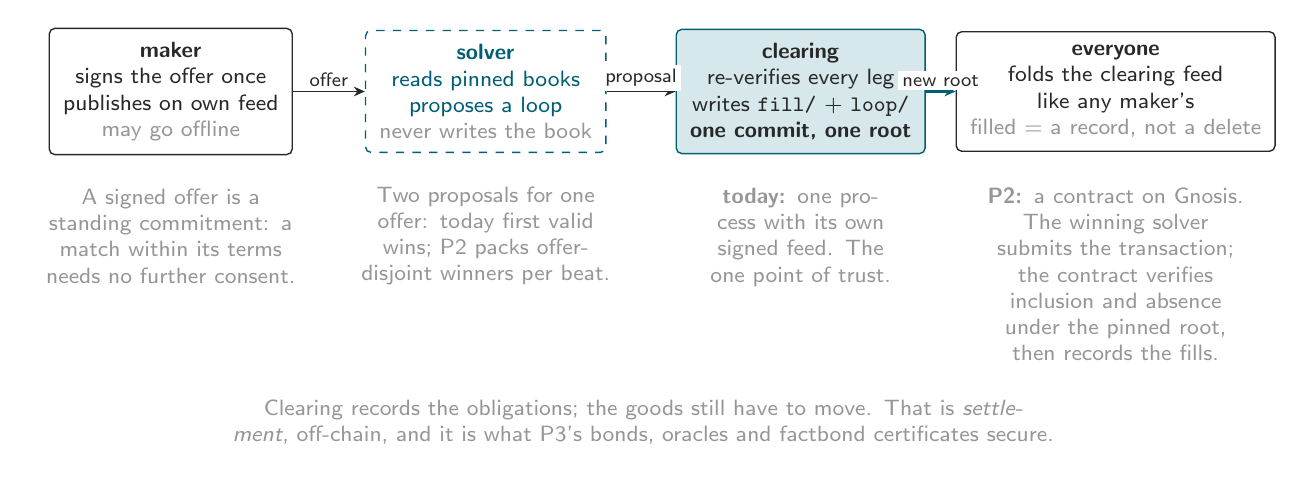
\begin{tikzpicture}[role/.style={box, align=center, font=\footnotesize, minimum width=30mm, minimum height=13mm}]
  % Who does what to the book. Makers sign once and may go offline; solvers
  % only propose; clearing is the one writer of fills; everyone folds.
  \node[role] (M) at (0,0) {\textbf{maker}\\ signs the offer once\\ publishes on own feed\\ {\color{soft}may go offline}};
  \node[role, dashed, draw=accent, text=accent] (S) at (40mm,0) {\textbf{solver}\\ reads pinned books\\ proposes a loop\\ {\color{soft}never writes the book}};
  \node[role, fill=accentlight, draw=accent] (T) at (80mm,0) {\textbf{clearing}\\ re-verifies every leg\\ writes \texttt{fill/} + \texttt{loop/}\\ \textbf{one commit, one root}};
  \node[role] (R) at (120mm,0) {\textbf{everyone}\\ folds the clearing feed\\ like any maker's\\ {\color{soft}filled = a record, not a delete}};
  \draw[flow] (M) -- node[lbl, above, font=\scriptsize] {offer} (S);
  \draw[flow] (S) -- node[lbl, above, font=\scriptsize] {proposal} (T);
  \draw[strong] (T) -- node[lbl, above, font=\scriptsize] {new root} (R);
  \node[note, text width=30mm, below=3mm of T] {\textbf{today:} one process with its own signed feed. The one point of trust.};
  \node[note, text width=34mm, below=3mm of T, xshift=40mm] {\textbf{P2:} a contract on Gnosis. The winning solver submits the transaction; the contract verifies inclusion and absence under the pinned root, then records the fills.};
  \node[note, text width=34mm, below=3mm of S] {Two proposals for one offer: today first valid wins; P2 packs offer-disjoint winners per beat.};
  \node[note, text width=34mm, below=3mm of M] {A signed offer is a standing commitment: a match within its terms needs no further consent.};
  \node[note, text width=128mm] at (60mm,-42mm) {Clearing records the obligations; the goods still have to move. That is \emph{settlement}, off-chain, and it is what P3's bonds, oracles and factbond certificates secure.};
\end{tikzpicture}
\end{document}
